% !TeX spellcheck = pt_PT
%
%
% Capítulo 2
%
\chapter{Formulação do Problema} \label{cap:formulacao}

Este capítulo está organizado em três secções, onde se descreve a formulação do problema e as suas especificações funcionais, assim como a arquitectura da solução.\\

\section{Formulação}\label{sec21}
Esta secção aborda todos os aspetos referentes à Formulação do Problema.\\

\begin{tabular}{ll}
	Tema: & Aplicação de Suporte a Equipas de Rugby \\
	Problema : & As equipas técnicas de Rugby têm ferramentas de suporte à sua organização? \\
		&	Que aspetos são necessários implementar numa aplicação para garantir \\
		&	esse suporte?\\
	%Problema v2: & Que aspectos são necessários implementar numa aplicação para garantir \\
		%&	a cobertura da falta de ferramentas de apoio às equipas técnicas de Rugby?\\
\end{tabular}\\[10mm]
A hipótese de resposta a esta pergunta foi adquirida da noção pessoal dos estudantes, como indivíduos com ligações interpessoais com o desporto, e das ideias que resultaram do diálogo com as duas equipas referidas neste documento. Após diversas reuniões com foco na recolha de ideias, foi atingida a hipótese de resposta descrita na secção 1.2. Apesar do problema apresentar algum teor subjetivo (equipas distintas operam e organizam-se de formas distintas, e sentem necessidades distintas em fatores distintos), foi possível alcançar uma solução que aglomera os fatores mais importantes para garantir a utilidade e a cobertura necessárias no contexto desta aplicação.

\section{Especificações Funcionais}\label{sec22}
Esta secção enumera as especificações funcionais da nossa solução, separando-as em especificações principais e especificações secundárias.

\subsection{Especificações Principais} \label{sec221}
A primeira sub-secção desta secção lista todos os conceitos chave que se pretendem desenvolver como espeficiações principais:
\begin{enumerate}
	\item Perfil de Atleta;
	\item Perfil de Equipa Técnica;
	\item Jogo;
	\item Estatísticas de Jogo;
	\item Treino;
	\item Planos de Treinos Físicos;
	\item Calendário de Eventos;
	\item Torneio;
	\item Evento;
\end{enumerate}

Estes conceitos definem a estrutura da nossa aplicação. 

A nossa aplicação irá implementar um perfil de Atleta, onde se pode observar a informação correspondente do atleta, como a idade, peso, altura, posições, assim como as suas estatísticas ao longo da época. Também será possível observar uma lista dos jogos onde foi convocado, ligações para as suas estatísticas nos mesmos, e uma lista de treinos e eventos a que compareceu. A aplicação irá também implementar perfis dedicados aos integrantes das equipas técnicas, para adicionar alguma coesão sobre a informação global da equipa.

A nossa aplicação irá implementar um menu de jogo, com as estatísticas da equipa no contexto desse jogo, os jogadores convocados e titulares, o oponente, e comentários adicionais.

A nossa aplicação irá implementar um menu de treinos, com as datas e locais de treinos, a lista de comparecentes, e comentários adicionais. A lista de comparecentes irá conseguir diferenciar os atletas que compareceram como ativos no treino, os que compareceram sem participar no treino ou os que compareceram para outra atividade ligada ao treino, como treinos físicos e de recuperação de lesões.

A nossa aplicação irá implementar um menu de planos de treino, onde a equipa técnica poderá fazer \emph{upload} de planos de treino físicos ou de ginásio, e indicar as datas onde estes planos se devem concretizar e os atletas a quem os planos se dirigem.

A nossa aplicação irá implementar um calendário, onde irão estar demonstrados todos os jogos, treinos, torneios ou outros eventos adicionados pela equipa técnica e a sua respetiva data de concretização.



\subsection{Especificações Secundárias} \label{sec222}
 Nesta secção apresentam-se algumas especificações secundárias. Conforme a disponibilidade, são especificações que poderão ser inseridas no contexto da aplicação, nomeadamente:
\begin{enumerate}
	\item Fisioterapeuta;
	\item Lesão;
	\item Campeonato;
	\item Estatísticas Gráficas;
	\item Exportação de Dados;
\end{enumerate}

Estes conceitos refletem a possibilidade de monitorizar e documentar lesões, e apresentá-las de forma organizada numa interface própria para uso pelos fisioterapeutas, assim como de organizar os diversos jogos da época num campeonato com respetivas classificações. Também propõe a possibilidade de exportar dados em formatos de texto para serem consumidos por outros meios, assim como de representar visualmente as estatísticas dos jogos com auxilio gráfico.

\section{Arquitetura da Solução}\label{sec23}
Esta secção explicita a arquitetura da nossa solução.

\begin{figure}[h]
	\begin{center}
		\resizebox{150mm}{!}{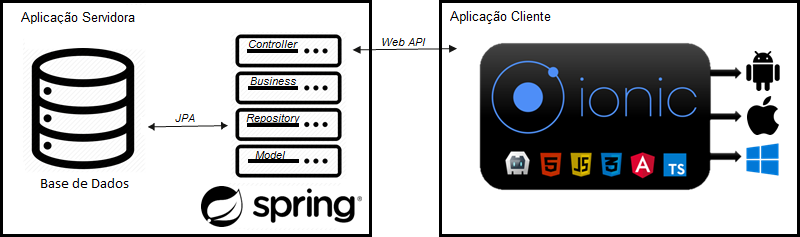
\includegraphics{./figures/arquitetura.png}}
	\end{center}
	\caption{Arquitetura da nossa solução.}\label{fig:arquitetura}
\end{figure}

O nosso projeto irá ser dividido entre aplicação servidora e aplicação cliente.

A aplicação servidora irá ser programada em \emph{Java} com uso da \emph{Spring Boot framework}. A base de dados irá ser programada em \emph{MySQL} com a ligação entre estes componentes feitos com o auxilio de \emph{JPA - Java Persistence API}. As diferentes camadas da aplicação servidora são abordadas no capítulo 3.

A aplicação cliente irá ter ambas as vertentes \emph{Web} e \emph{mobile}, programadas em \emph{TypeScript}, com o uso de \emph{Angular framework} e \emph{IONIC framework}.

A camada \textit{Controller} da aplicação servidora expõe uma \textit{Web API}, e são as chamadas feitas a essa \textit{API} pelo lado da aplicação cliente que fazem a ligação entre as duas.

Entende-se que a maioria destes domínios sejam familiares ao leitor.

